\subsection{Configurazione Database}
Si è optato per l'utilizzo di \textit{ClickHouse}\textsubscript{\textit{G}} per il salvataggio dei dati, le motivazioni sono descritte nella sezione \ref{sec:clickHouse}. In particolare, per ogni \textit{sensore}\textsubscript{\textit{G}} di cui si desidera memorizzare le misurazioni, viene creata una tabella che le acquisisce dal relativo topic \textit{Kafka}\textsubscript{\textit{G}} e una tabella della famiglia MergeTree che permette la loro persistenza.
Le tipologie di sensori le quali misurazioni si vogliono trattare nel progetto sono:
\begin{itemize}
    \item Sensori di temperatura;
    \item Sensori di umidità;
    \item Sensori di rilevamento polveri sottili; 
    \item Sensori di stato di riempimento delle isole ecologiche;
    \item Sensori di occupazione delle colonnine di ricarica;
    \item Sensori di guasti elettrici;
    \item Sensori di presenza dell'acqua.
\end{itemize}
Oltre alla misurazioni dei sensori, si è deciso di memorizzare in una tabella apposita anche i punteggi di salute calcolati per ogni cella sulla base delle relative misurazioni.

La progettazione del \textit{database}\textsubscript{\textit{G}} \textit{ClickHouse}\textsubscript{\textit{G}} è cruciale, poiché un'adeguata ottimizzazione consente di garantire prestazioni ottimali per un \textit{sistema}\textsubscript{\textit{G}} orientato al tempo reale e che richiede analisi su grandi volumi di dati.

\subsubsection{Funzionalità Clickhouse utilizzate}
\paragraph{Materialized Views}
\textbf{Documentazione:}

\url{https://clickhouse.com/docs/en/guides/developer/cascading-materialized-views} (Consultato 25/03/2024).\newline
Le Materialized Views in \textit{ClickHouse}\textsubscript{\textit{G}} sono un meccanismo volto a migliorare le prestazioni delle \textit{query}\textsubscript{\textit{G}} e semplificare l'accesso ai dati.

Funzionano mantenendo una copia fisica dei risultati di una \textit{query}\textsubscript{\textit{G}} di selezione, che viene quindi memorizzata su disco. Questa copia è aggiornata periodicamente in base ai dati sottostanti.

\paragraph{Utilizzi principali delle Materialized Views}
\begin{itemize}
    \item \textbf{Calcolo aggregazioni e popolamento tabelle:} Le materialized Views vengono utilizzate per calcolare aggregazioni su dati e quindi popolare altre tabelle con i risultati aggregati;
    \item \textbf{Ottimizzazione delle prestazioni:} Memorizzando i risultati di una \textit{query}\textsubscript{\textit{G}} complessa, le Materialized Views consentono di eseguire rapidamente le \textit{query}\textsubscript{\textit{G}} successive senza dover ricalcolare i dati ogni volta. Ciò è particolarmente utile in applicazioni che richiedono interrogazioni frequenti su grandi volumi di dati;
    \item \textbf{Decomposizione delle query complesse:} Le Materialized Views consentono di decomporre \textit{query}\textsubscript{\textit{G}} complesse in passaggi più semplici e riutilizzabili, migliorando la leggibilità del codice e semplificando lo sviluppo e la manutenzione delle \textit{query}\textsubscript{\textit{G}}.
\end{itemize}

Nel progetto le materialized view sono fondamentali per spostare automaticamente i dati dai topic \textit{Kafka}\textsubscript{\textit{G}} alle tabelle di destinazione.
\begin{figure}[H]
  \centering
  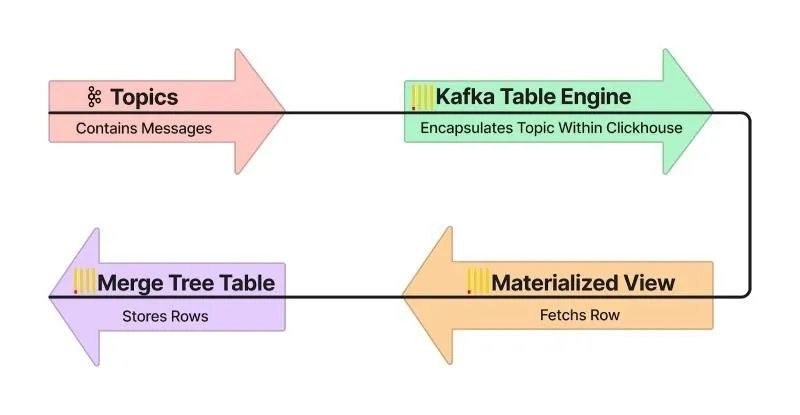
\includegraphics[width=1\textwidth]{../Images/SpecificaTecnica/enginePipeline.jpg}
  \caption{Clickhouse data pipeline}
  \label{fig:data_pipeline_clickhouse}
\end{figure}

\paragraph{MergeTree}\label{sec:MergeTree}
\textbf{Documentazione:}

\url{https://clickhouse.com/docs/en/engines/table-engines/mergetree-family/mergetree#mergetree} (Consultato 25/03/2024).\newline
MergeTree è uno dei motori di archiviazione di base più utilizzati in \textit{ClickHouse}\textsubscript{\textit{G}}. È progettato per gestire dati ordinati in \textit{append-only} e offre un'ottima combinazione di prestazioni di lettura, scrittura, scalabilità e funzionalità per diversi casi d'uso.

Caratteristiche principali:
\begin{itemize}
	\item \textbf{Ordinato:} I dati sono archiviati in ordine crescente in base alla chiave di ordinamento specificata;
	\item \textbf{Append-only:} I nuovi dati vengono sempre aggiunti alla fine della tabella;
	\item \textbf{Scalabile:} Altamente scalabile orizzontalmente;
	\item \textbf{Partizionamento:} Supporto per partizionare la tabella in base a una colonna specifica;
	\item \textbf{TTL (Time to Live):} Consente di definire un TTL per i dati, eliminandoli automaticamente dopo un periodo di tempo specificato;
	\item \textbf{Compressione:} Supporta diverse tecniche di compressione per ridurre lo spazio di archiviazione utilizzato.
\end{itemize}

\textbf{Casi d'uso comuni:}
\begin{itemize}
  \item Analisi di \textit{log}\textsubscript{\textit{G}};
  \item Dati finanziari;
  \item Dati di monitoraggio;
  \item Time series data.
\end{itemize}

\textbf{Vantaggi:}
\begin{itemize}
  \item Prestazioni di lettura e scrittura elevate;
  \item Scalabilità orizzontale;
  \item Funzionalità avanzate;
  \item Adatto a diversi casi d'uso.
\end{itemize}

\paragraph{Time to Live in ClickHouse} \label{sec:RollupTTL}
\textbf{Documentazione:}

\url{https://clickhouse.com/docs/en/guides/developer/ttl#implementing-a-rollup}\newline

TTL \textit{(Time To Live)} si riferisce alla capacità di spostare, eliminare o eseguire il rollup di righe o colonne dopo che è trascorso un determinato intervallo di tempo. Sebbene l'espressione "time to live" sembri applicarsi solo all'eliminazione di vecchi dati, TTL ha diversi casi d'uso:

\begin{itemize}
	\item \textbf{Eliminazione dei vecchi dati:} Rimuovere i dati dopo un certo periodo di tempo;
	\item \textbf{Spostamento dei dati tra dischi:} Spostare i dati tra volumi di archiviazione dopo un certo periodo di tempo;
	\item \textbf{Rollup dei dati:} Effettuare operazioni di aggregazione sui dati dopo un intervallo di tempo prestabilito.
\end{itemize}

Nel progetto è stato fatto utilizzo dove opportuno dell'operazione di Rollup di misurazioni dei sensori.
Nello specifico dopo un certo intervallo di tempo non vengono piu conservate tutte le misurazioni di ogni \textit{sensore}\textsubscript{\textit{G}}, ma solo la media delle loro misurazioni nel periodo di tempo specificato. Questo permette di ridurre il volume di dati da analizzare e di mantenere comunque un'informazione utile per l'analisi.

\paragraph{Partition}\label{sec:Partition}
\textbf{Documentazione:}

\url{https://clickhouse.com/docs/en/engines/table-engines/mergetree-family/mergetree#partition-by} (Consultato 25/03/2024).

Le partizioni sono una funzionalità fondamentale di \textit{ClickHouse}\textsubscript{\textit{G}} che consente di organizzare in modo efficiente la gestione di grandi volumi di dati. Questa funzionalità permette di suddividere i dati in gruppi logici in base a criteri specifici, come il valore di una colonna o un intervallo di tempo.

Grazie a questa organizzazione ottimizzata, le \textit{query}\textsubscript{\textit{G}} che richiedono l'accesso a dati specifici all'interno di una partizione possono essere eseguite rapidamente, garantendo prestazioni elevate anche su dataset di grandi dimensioni.

Le partizioni rappresentano uno strumento particolarmente utile quando si lavora con dati di serie temporali. La decisione sull'utilizzo del partizionamento dovrebbe derivare da una serie di considerazioni chiave:

\begin{itemize}
	\item \textbf{Interrogazione singola:} È previsto che le \textit{query}\textsubscript{\textit{G}} siano principalmente focalizzate su una singola partizione? Ad esempio, se le interrogazioni tendono a riguardare risultati entro un periodo specifico come un giorno o un mese, sarebbe vantaggioso partizionare i dati in base a tali periodi temporali.
	\item \textbf{Scadenza dei dati (TTL):} Se si desidera applicare una politica di TTL ai dati, in modo che una volta che una partizione raggiunge una certa età, venga applicata un'azione specifica su di essa, allora può risultare opportuno l'utilizzo del partitioning in base a tali periodi temporali.
\end{itemize}

Spesso si consiglia di mantenere il numero di partizioni al di sotto di circa 100. Anche se è tecnicamente possibile utilizzare fino a 1000 partizioni, tale approccio potrebbe non essere ottimale e potrebbe influenzare le prestazioni del \textit{sistema}\textsubscript{\textit{G}}, inclusi tempi di avvio, tempi di inserimento, \textit{query}\textsubscript{\textit{G}}-time e l'utilizzo di memoria.

Questo è dovuto all'impatto che un elevato numero di partizioni può avere sul file system e sulle dimensioni dell'indice, con conseguente aumento della complessità gestionale e dei carichi di lavoro.

Nel nostro progetto viene fatto utilizzo del partizionamento temporale nelle tabelle in cui è ritenuto oppurtuno sulla base delle considerazioni sopra descritte. L'utilizzo viene giustificato infatti dall'impiego di TTL, oltre al fatto che le interrogazioni riguardino principalmente una singola partizione.
    
\paragraph{Projection}\label{sec:projections}
\textbf{Documentazione:}

\url{https://clickhouse.com/docs/en/sql-reference/statements/alter/projection} (Consultato 25/03/2024).

\textbf{Approfondimento:} \url{https://presentations.clickhouse.com/percona2021/projections.pdf} (Consultato 25/03/2024).

Le projection in \textit{ClickHouse}\textsubscript{\textit{G}} sono una funzionalità di ottimizzazione per migliorare le prestazioni delle \textit{query}\textsubscript{\textit{G}} su tabelle MergeTree. Esse creano delle viste pre-aggregate o pre-ordinate dei dati originali, consentendo a \textit{ClickHouse}\textsubscript{\textit{G}} di accedere e analizzare i dati in modo più efficiente.

Questa funzionalità è utile per:

\begin{itemize}
    \item Eseguire \textit{query}\textsubscript{\textit{G}} basate su di una colonna che non fa parte della chiave primaria;
    \item Pre-aggregare colonne, riducendo sia i calcoli che l'I/O.
\end{itemize}

Come funzionano le projection:
\begin{itemize}
	\item \textbf{Definizione:} Si definisce una projection su una tabella MergeTree esistente. La projection specifica una sottocategoria di colonne e, opzionalmente, un nuovo ordine di ordinamento per queste colonne;
	\item \textbf{Creazione interna:} \textit{ClickHouse}\textsubscript{\textit{G}} crea internamente una nuova tabella nascosta che contiene i dati della projection;
	\item \textbf{Aggregazione o ordinamento:} I dati selezionati vengono aggregati (utilizzando funzioni come media, somma, ecc.) o ordinati in base alle colonne specificate nella definizione della projection;
	\item \textbf{Selezione automatica:} Durante l'esecuzione di una \textit{query}\textsubscript{\textit{G}}, \textit{ClickHouse}\textsubscript{\textit{G}} analizza la projection e la tabella originale. Se la projection rientra nei criteri di selezione della \textit{query}\textsubscript{\textit{G}} (colonne e ordine), \textit{ClickHouse}\textsubscript{\textit{G}} può utilizzare la projection per rispondere alla \textit{query}\textsubscript{\textit{G}}, evitando di accedere alla tabella originale completa.
\end{itemize}

Vantaggi delle projection:
\begin{itemize}
	\item \textbf{Miglioramento delle prestazioni:} Accedendo ai dati pre-aggregati o pre-ordinati, le \textit{query}\textsubscript{\textit{G}} possono essere eseguite più velocemente;
	\item \textbf{Riduzione dell'utilizzo della CPU:} Le aggregazioni e gli ordinamenti vengono eseguiti durante la creazione della projection, riducendo il carico di lavoro della CPU durante le \textit{query}\textsubscript{\textit{G}};
	\item \textbf{Più flessibilità di query:} Le projection possono supportare ordini diversi rispetto alla tabella originale, aumentando la flessibilità delle \textit{query}\textsubscript{\textit{G}}.
\end{itemize}

Nel contesto del progetto, le projection sono state impiegate strategicamente al fine di ottimizzare le prestazioni delle interrogazioni basate sulla colonna "\textit{cella}". Questa colonna, pur non facendo parte della chiave primaria, è oggetto di interrogazioni molto frequenti su vasti volumi di dati.

L'utilizzo di tale strategia si rivela particolarmente vantaggiosa vista la previsione di interrogazioni ricorrenti e su dataset di grandi dimensioni basate su tale colonna, contribuendo così a garantire tempi di risposta ottimizzati e una migliore esperienza utente.

In generale l'introduzione delle projections produce risultati di notevole importanza, come illustrato di seguito.

Consideriamo una \textit{query}\textsubscript{\textit{G}}, che calcola la media globale di \textbf{170'000} misurazioni di temperatura tramite \textit{Grafana}\textsubscript{\textit{G}}:

\begin{lstlisting}[caption={Esempio query - Grafana}, captionpos=b]
	SELECT avgMerge(value) count(*)
	FROM innovacity.temperatures
	WHERE cella = 'Arcella'

	--\textit{Query}\textsubscript{\textit{G}} id: 59811218-6f57-4753-b24a-a81c2a8380df
\end{lstlisting}

Senza l'utilizzo delle projections, il risultato ottenuto è il seguente:

\begin{figure}[H]
    \centering
    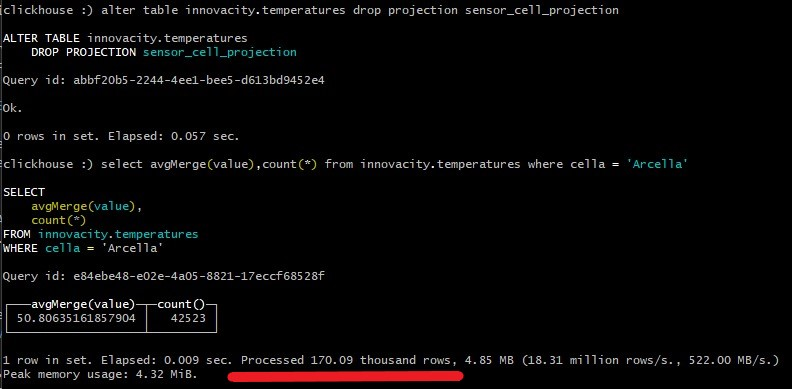
\includegraphics[width=1\textwidth]{../Images/SpecificaTecnica/query2ProjectionsWithout.jpg}
    \caption{Query esempio senza projection - ClickHouse}
    \label{fig:without2proj}
  \end{figure}

Il totale di righe processate per ottenere il risultato è  \textbf{170'090}, ovvero la totalità delle righe presenti nella tabella, con \textbf{9}ms di tempo utilizzati e un picco di memoria RAM impiegata di \textbf{4.32}MiB.

Con l'impiego delle projections invece il risultato ottenuto è il seguente:

\begin{figure}[H]
    \centering
    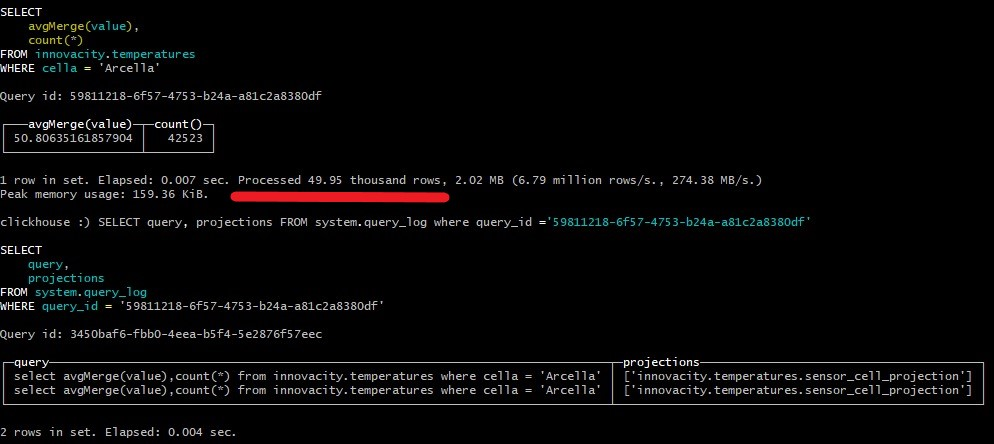
\includegraphics[width=1\textwidth]{../Images/SpecificaTecnica/query2ProjectionsWith.jpg}
    \caption{Query esempio projection - ClickHouse}
    \label{fig:with2proj}
\end{figure}

Il totale di righe processate per ottenere il risultato è di \textbf{49'950} con \textbf{7}ms di tempo utilizzati e un picco di memoria RAM impiegata di \textbf{159.36}KiB.

\subsubsection{Integrazione Kafka tramite Kafka Engine in ClickHouse}\label{sec:kafka_engine}

\textit{ClickHouse}\textsubscript{\textit{G}} supporta l'\textit{integrazione}\textsubscript{\textit{G}} con \textit{Kafka}\textsubscript{\textit{G}} tramite \textit{Kafka}\textsubscript{\textit{G}} Engine, permettendo la lettura dei dati da un topic \textit{Kafka}\textsubscript{\textit{G}} e il loro salvataggio in una tabella \textit{ClickHouse}\textsubscript{\textit{G}} adatta a grandi dataset. Tale funzionalità riveste un'importanza notevole per applicazioni che richiedono l'elaborazione in tempo reale di dati provenienti da fonti esterne, una necessità frequente nel contesto del monitoraggio urbano. L'\textit{integrazione}\textsubscript{\textit{G}} con \textit{Kafka}\textsubscript{\textit{G}} consente l'acquisizione e la memorizzazione efficiente di dati, anche in grosse quantità, garantendo comunque prestazioni elevate.

\textit{Kafka}\textsubscript{\textit{G}} Engine è progettato per il recupero di dati una sola volta. Ciò significa che una volta che i dati vengono interrogati da una tabella \textit{Kafka}\textsubscript{\textit{G}}, vengono considerati consumati dalla coda. Pertanto, non si dovrebbero mai selezionare dati direttamente da una tabella di \textit{Kafka}\textsubscript{\textit{G}} Engine, ma utilizzare invece una Materialized View.

Una Materialized View viene attivata una volta che i dati sono disponibili in una tabella di \textit{Kafka}\textsubscript{\textit{G}} Engine. Automaticamente i dati vengono spostati da una tabella \textit{Kafka}\textsubscript{\textit{G}} a una tabella di tipo MergeTree o Distributed.

Sono quindi necessarie almeno 3 tabelle:

\begin{itemize}
  \item La tabella di origine del \textit{Kafka}\textsubscript{\textit{G}} Engine;
  \item La tabella di destinazione (MergeTree o Distributed);
  \item Materialized View per spostare i dati.
\end{itemize}

\begin{figure}[H]
	\centering
	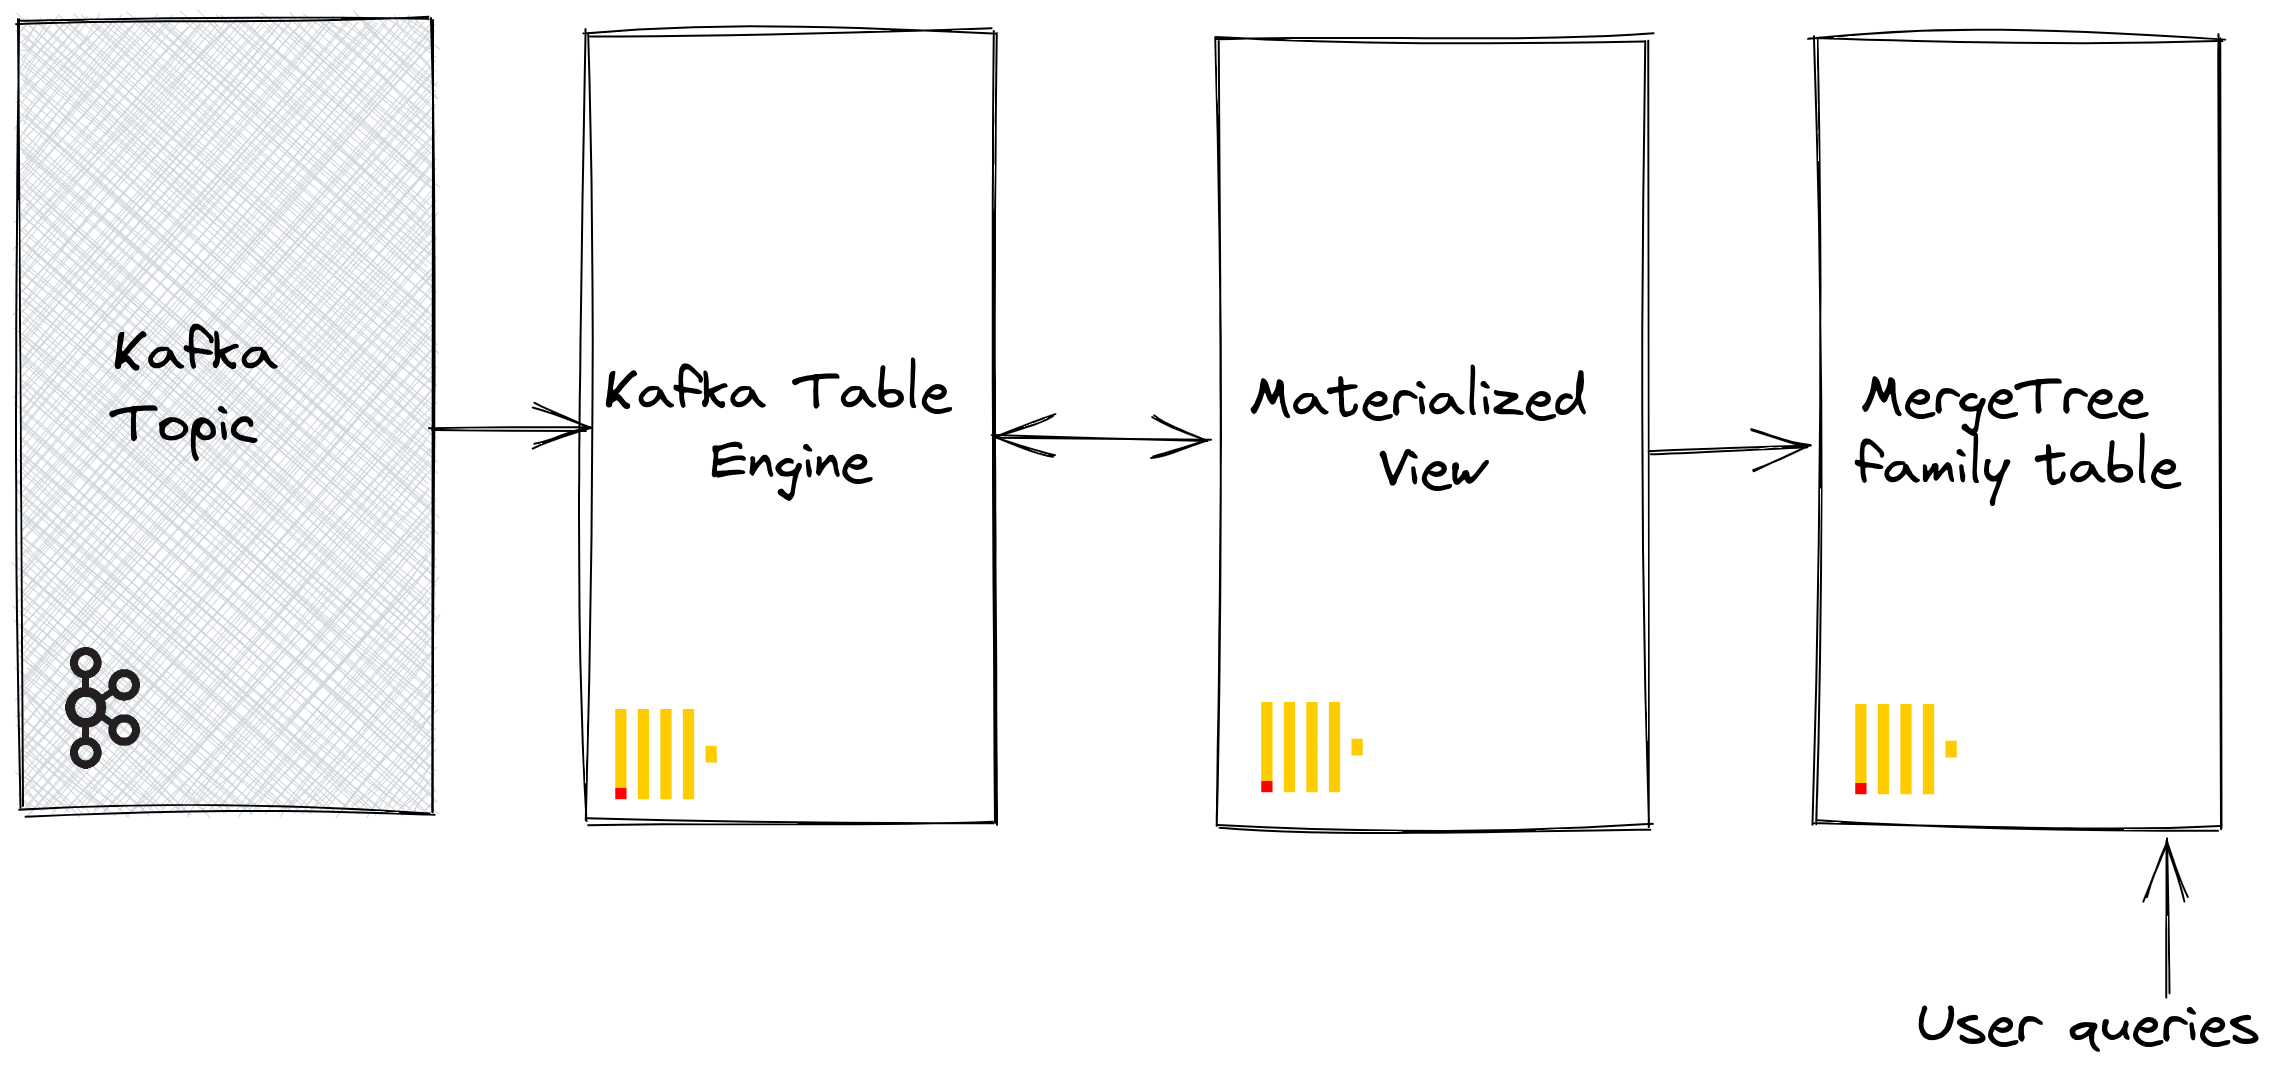
\includegraphics[width=.7\textwidth]{../Images/SpecificaTecnica/kafka_engine_architecture.png}
	\caption{Architettura di Kafka Engine in ClickHouse}
	\label{fig:Architettura_kafka_engine}
\end{figure}

\subsubsection{Trasferimento dati tramite Materialized View} \label{sec:materializedView}

Una materialized view funge da ponte tra la fonte dei dati (\textit{Kafka}\textsubscript{\textit{G}} Engine) e la destinazione dei dati (MergeTree). Quando nuovi dati vengono scritti nella tabella \textit{Kafka}\textsubscript{\textit{G}} Engine, la materialized view viene attivata automaticamente.

La materialized view esegue una \textit{query}\textsubscript{\textit{G}} sulla tabella \textit{Kafka}\textsubscript{\textit{G}} Engine per selezionare i dati più recenti. Una volta selezionati, questi dati vengono inseriti nella tabella di destinazione (ad esempio, una tabella MergeTree). Questo processo avviene in modo automatico e immediato, senza bisogno di intervento manuale.

In pratica, la materialized view si assicura che la tabella di destinazione sia sempre aggiornata con i dati più recenti presenti nella tabella \textit{Kafka}\textsubscript{\textit{G}} Engine.

Questo offre numerosi vantaggi:
\begin{itemize}
	\item \textbf{Automatizzazione del processo:} Non è necessario eseguire manualmente operazioni di trasferimento dati da una tabella all'altra. La materialized view si occupa di tutto in modo automatico;
	\item \textbf{Efficienza:} Il trasferimento dei dati avviene in tempo reale, garantendo che la tabella di destinazione sia sempre allineata con la fonte dei dati senza ritardi;
	\item \textbf{Ottimizzazione delle risorse:} Il processo di trasferimento dei dati è gestito in modo efficiente, utilizzando al meglio le risorse disponibili e garantendo prestazioni elevate.
\end{itemize}

Nel contesto specifico, le materialized view sono responsabili di eseguire controlli sui dati, come ad esempio la verifica della loro correttezza ed affidabilità nel contesto di utilizzo, prima di inserirli nella tabella di destinazione.

Questo processo assicura che i dati siano sempre affidabili e pronti per l'analisi, senza la necessità di ulteriori operazioni di pulizia o preparazione.

Per esempio, nel caso dei dati di umidità raccolti da sensori in un'area urbana, la materialized view potrebbe eseguire controlli per assicurarsi che i valori rientrino all'interno di un intervallo plausibile e che non ci siano discrepanze improbabili. Ciò garantirebbe che i dati di umidità inseriti nella tabella di destinazione siano accurati e affidabili per l'analisi meteorologica o ambientale.

\subsubsection{Tabella Kafka Engine per un sensore generico}
Le tabelle del \textit{database}\textsubscript{\textit{G}} impiegate per ottenere le misurazioni di ciascuna tipologia di \textit{sensore}\textsubscript{\textit{G}} dai topic \textit{kafka}\textsubscript{\textit{G}} presentano una configurazione sostanzialmente simile, differenziandosi principalmente per il tipo di dato della colonna relativa alla misurazione e per il \textit{topic} di riferimento utilizzato per ottenere le misurazioni.

Nello specifico per ogni \textit{sensore}\textsubscript{\textit{G}} si avrà la seguente tabella \textit{Clickhouse}\textsubscript{\textit{G}}:
\begin{figure}[H]
    \centering
    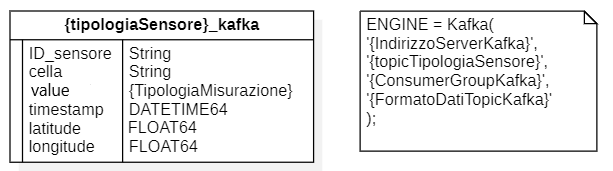
\includegraphics[width=.6\textwidth]{../Images/SpecificaTecnica/sensorType_kafka.PNG}
    \caption{Tabella sensore generico per il reperimento da Kafka - ClickHouse}
    \label{fig:Reperimento_kafka_clickhouse}
  \end{figure}

La tabella è configurata con il motore di \textit{storage}\textsubscript{\textit{G}} \textit{Kafka}\textsubscript{\textit{G}}, il che significa che i dati verranno letti direttamente da un topic \textit{Kafka}\textsubscript{\textit{G}}. 

I campi sono:
\begin{itemize}
	\item \textbf{ID\_sensore:} Un campo di tipo \textit{String} che identifica univocamente il \textit{sensore}\textsubscript{\textit{G}} che ha effettuato la misurazione;
	\item \textbf{cella:} Un campo di tipo \textit{String} che rappresenta la cella della città in cui è stata effettuata la misurazione;
	\item \textbf{value:} Un campo di tipo variabile a seconda del tipo di misurazione;
	\item \textbf{timestamp:} Un campo di tipo \textit{DATETIME64} che rappresenta il timestamp della misurazione;
	\item \textbf{latitude:} Un campo di tipo \textit{Float64} che rappresenta la latitudine del luogo dove è stata effettuata la misurazione;
	\item \textbf{longitude:} Un campo di tipo \textit{Float64} che rappresenta la longitudine del luogo dove è stata effettuata la misurazione.
\end{itemize}

Mentre i parametri esposti racchiusi da parentesi graffe variano per ogni tipolgia di \textit{sensore}\textsubscript{\textit{G}} correlato alla misurazione e sono:

\begin{itemize}
	\item \textbf{tipologiaSensore:} Viene sostituito con la tipologia del \textit{sensore}\textsubscript{\textit{G}} che effettua le misurazioni salvate nella tabella (ex. temperatures);
	\item \textbf{TipologiaMisurazione:} Viene sostituito con il tipo del dato che rappresenta la misurazione;
	\item \textbf{IndirizzoServerKafka:} Specifica l'indirizzo del server \textit{Kafka}\textsubscript{\textit{G}}. Nel nostro caso il server è in esecuzione su un \textit{container}\textsubscript{\textit{G}} \textit{Docker} raggiungibile tramite l'indirizzo: \textit{'kafka:9092'};
	\item \textbf{topicTipologiaSensore:} Specifica il nome del topic \textit{Kafka}\textsubscript{\textit{G}} da cui leggere i dati (ex.temperature). Accetta anche liste di topic \textit{Kafka}\textsubscript{\textit{G}} separati da virgole;
	\item \textbf{ConsumerGroupKafka:} Specifica il nome del consumer group \textit{Kafka}\textsubscript{\textit{G}} che verrà utilizzato per leggere i messaggi dal topic \textit{Kafka}\textsubscript{\textit{G}}.
	Un consumer group in \textit{Kafka}\textsubscript{\textit{G}} è un gruppo di consumatori che lavorano insieme per consumare i messaggi da uno o più topic. Ogni messaggio inviato a un topic \textit{Kafka}\textsubscript{\textit{G}} può essere consumato da uno dei consumatori nel gruppo.
	
	I consumer all'interno di uno stesso gruppo condividono l'elaborazione dei messaggi all'interno dei topic: ogni messaggio viene elaborato da uno e un solo consumatore all'interno del gruppo. Nel nostro caso sarà sempre '\textit{CG\_Clickhouse\_1}' per indicare il \textit{servizio}\textsubscript{\textit{G}} di salvataggio \textit{Clickhouse};
	\item \textbf{FormatoDatiTopicKafka:} specifica il formato dei dati nel topic \textit{Kafka}\textsubscript{\textit{G}}. Nel nostro caso, i dati sono nel formato JSONEachRow, che è un formato di serializzazione JSON di \textit{ClickHouse} che consente di scrivere o leggere record JSON separati da una riga;


\item \textbf{KafkaSkipBrokenMessages:}
\begin{itemize}
	\item è un'opzione di configurazione utilizzata nell'Engine \textit{Kafka}\textsubscript{\textit{G}} di \textit{ClickHouse}\textsubscript{\textit{G}}. Determina il comportamento dell'Engine quando incontra messaggi \textit{Kafka}\textsubscript{\textit{G}} considerati "corrotti" o non processabili.
	Un messaggio \textit{Kafka}\textsubscript{\textit{G}} può essere considerato corrotto per diversi motivi, tra cui:
	\begin{itemize}
		\item \textbf{Formato non valido:} Il messaggio potrebbe avere un formato JSON o Avro non valido, impedendo a \textit{ClickHouse}\textsubscript{\textit{G}} di decodificarlo correttamente;
		\item \textbf{Dati mancanti:} Il messaggio potrebbe contenere dati mancanti o incompleti, violando lo schema previsto;
		\item \textbf{Errori di codifica:} Il messaggio potrebbe avere errori di codifica che impediscono la lettura dei dati.
	\end{itemize}
	\item Per impostazione predefinita, \textit{kafka\_skip\_broken\_messages} è impostato su 0. Ciò significa che \textit{ClickHouse}\textsubscript{\textit{G}} interrompe l'elaborazione del flusso di dati da \textit{Kafka}\textsubscript{\textit{G}} e registra un errore quando incontra un messaggio corrotto;
	\item Puoi configurare \textit{kafka\_skip\_broken\_messages} su un valore diverso da zero per modificare il comportamento. Il valore rappresenta il numero massimo di messaggi corrotti consecutivi per blocco, considerato nel contesto di  \textit{kafka\_max\_block\_size}, che \textit{ClickHouse}\textsubscript{\textit{G}} ignorerà prima di interrompere l'elaborazione;
	\item Bisogna anche ricordare che per come è stato progettato il \textit{sistema}\textsubscript{\textit{G}} i messaggi corrotti vengono scartati "alla fonte" dallo Schema Registry di \textit{Kafka}\textsubscript{\textit{G}};
	\item Nel nostro caso vogliamo che ogni messaggio malformato nel blocco venga ignorato.
\end{itemize}
\item \textbf{input\_format\_skip\_unknown\_fields}:  è un'impostazione utilizzata con alcuni formati di input di \textit{ClickHouse}\textsubscript{\textit{G}}, compreso quello da noi utilizzato \textit{JSONEachRow} per specificare come gestire i dati in entrata che contengono colonne sconosciute alla tabella di destinazione. Impostando \textit{input\_format\_skip\_unknown\_fields} su 1, \textit{ClickHouse}\textsubscript{\textit{G}} ignorerà le colonne sconosciute nei dati in entrata e importerà solo le colonne corrispondenti alla tabella di destinazione. Questo è utile quando si desidera importare solo una parte dei dati in entrata, ignorando le colonne non necessarie o non rilevanti.
Nel nostro caso l'impostazione di default è quella richiesta.
\end{itemize}


\subsubsection{Misurazioni temperatura} \label{sec:misurazioni_temperatures}

Di seguito viene presentata una configurazione dettagliata per l'archiviazione delle misurazioni di temperatura. Tale configurazione, progettata per acquisire dati da un topic \textit{Kafka}\textsubscript{\textit{G}} permette la persistenza delle misurazioni di temperatura che include l'\textit{ID}\textsubscript{\textit{G}} del \textit{sensore}\textsubscript{\textit{G}} (String), la cella della città da cui proviene la misurazione (String), la temperatura misurata (Float32), il timestamp della misurazione (DATETIME64), la latitudine (Float64) e la longitudine (Float64) del \textit{sensore}\textsubscript{\textit{G}}.

La tabella di destinazione è denominata temperatures e utilizza il motore di \textit{storage}\textsubscript{\textit{G}} MergeTree, che è ottimizzato per l'archiviazione e l'analisi di dati cronologicamente ordinati in append-only. Questa scelta è giustificata dal fatto che le misurazioni di temperatura sono tipicamente ordinate cronologicamente.

Da osservare che l'attributo presente nel messaggio JSON : \textit{type} viene ignorato, poichè non necessario in una tabella dedicata alle sole misurazioni di temperatura. Ciò accade grazie al valore di deault dell'impostazione \textit{input\_format\_skip\_unknown\_fields} della tabella con Kakfa Engine.
Vengono definite come \textit{PRIMARY KEY} le colonne \textit{ID\_sensore} e \textit{timestamp} per garantire l'unicità delle misurazioni e la possibilità di effettuare ricerche efficienti.

\begin{figure}[H]
	\centering
	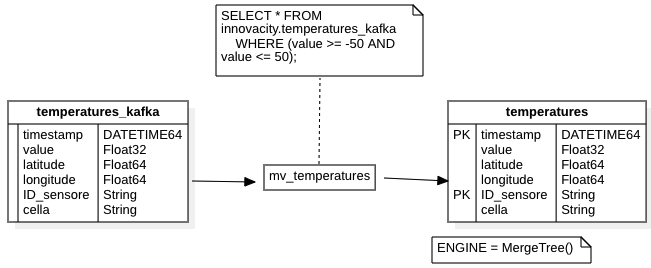
\includegraphics[width=1\textwidth]{../Images/SpecificaTecnica/temperatures.png}
	\caption{Tabella temperatures\_kafka e temperatures}
	\label{fig:temperatures}
\end{figure}
    
La tabella temperatures\_kafka come spiegato in precedenza funge da tramite tra il topic \textit{Kafka}\textsubscript{\textit{G}} relativo alle misurazioni di temperatura e il \textit{sistema}\textsubscript{\textit{G}} di gestione dei dati \textit{ClickHouse}\textsubscript{\textit{G}}.

Questa tabella agisce come un'interfaccia trasformando i flussi di dati provenienti dal topic \textit{Kafka}\textsubscript{\textit{G}} in un formato comprensibile per \textit{ClickHouse}\textsubscript{\textit{G}}. Successivamente, una Materialized View, in questo caso mv\_temperatures, opera su questa tabella per trasferire i dati ottenuti verso la tabella di destinazione temperatures della famiglia MergeTree come spiegato in \ref{sec:materializedView}.
    
\paragraph{Projections per misurazioni di temperatura} \label{sec:temp_projections}

Durante la fase di progettazione, è stata dedicata particolare attenzione all'utilizzo delle tabelle precedentemente descritte e alle richieste che verranno formulate su di esse. È emerso che, considerando il requisito di suddividere la città in una serie di celle e specificare la cella di origine della misurazione, la filtrazione delle misurazioni per celle diventerà una richiesta frequente al \textit{database}\textsubscript{\textit{G}}. Di conseguenza, si è optato per l'utilizzo delle projections per ottimizzare il filtering su tale campo, le quali sono dettagliatamente descritte nella sezione \ref{sec:projections}.
\vspace{0,3cm}
\begin{lstlisting}[caption={implementazione projection tabella temperatures}, captionpos=b]
  --Projection per tabella temperatures
	ALTER TABLE innovacity.temperatures ADD PROJECTION tmp_sensor_cell_projection (SELECT * ORDER BY cella);
	ALTER TABLE innovacity.temperatures MATERIALIZE PROJECTION tmp_sensor_cell_projection;
\end{lstlisting}

La proiezione ci consentirà di effettuare rapidamente filtraggi basati sulle celle, anche se tale attributo non è definito come \textit{PRIMARY\_KEY} nella tabella originale.
      
\paragraph{TTL per misurazioni di temperatura} \label{sec:temp_TTL}

L'implementazione del Time To Live \textit{(TTL)} di rollup per le misurazioni di temperatura deve permettere di salvare un solo dato aggregato per ora e per \textit{sensore}\textsubscript{\textit{G}} dopo che è trascorso più di un mese dal timestamp della misurazione.

\begin{lstlisting}[caption={implementazione TTL tabella temperatures}, captionpos=b]
    TTL toDateTime(timestamp) + INTERVAL 1 MONTH
	GROUP BY ID_sensore, toStartOfHour(timestamp)
	SET value = avg(value);
\end{lstlisting}

\paragraph{Partition per misurazioni di temperatura}\label{sec:temp_part}
La tabella è partizionata per anno e mese in base al valore della colonna timestamp. Ciò significa che i dati vengono archiviati in parti separate per ogni combinazione di anno e mese. Questo approccio consente di organizzare i dati in modo efficiente e di eseguire \textit{query}\textsubscript{\textit{G}} su intervalli temporali specifici in modo rapido ed efficiente. Inoltre, il partizionamento per anno e mese consente di applicare il TTL in modo selettivo.
La scelta sull'utilizzo delle Partition e sulla relativa configurazione è stata dettata dalle considerazioni esposte in \ref{sec:Partition}.


\subsubsection{Misurazioni umidità}
Le considerazioni relative al salvataggio delle misurazioni di umidità coincidono con quelle espresse nella sezione \ref{sec:misurazioni_temperatures} riguardo alle misurazioni di temperatura.
In questa situazione, dove le misure riguardano l’umidità, la tabella di destinazione \textit{ClickHouse}\textsubscript{\textit{G}} è nominata ‘humidity’:
Il tipo della colonna \textit{value} è \textit{Float32} poichè il valore dell'umidità è in percentuale, compreso tra 0 e 100. Le altre colonne sono identiche a quelle della tabella 'temperatures' e sono definite con lo stesso tipo di dato per garantire la precisione e l'integrità dei dati.
\begin{figure}[H]
    \centering
    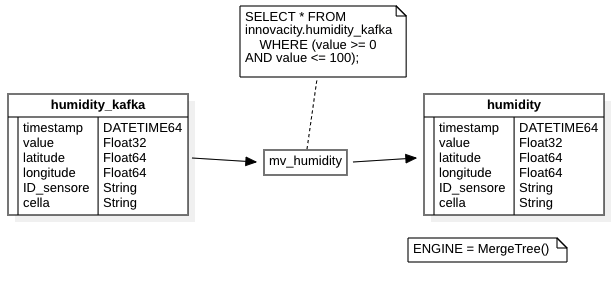
\includegraphics[width=1\textwidth]{../Images/SpecificaTecnica/humidity.png}
    \caption{Tabella humidity\_kafka e humidity}
    \label{fig:humidity_tables}
  \end{figure}

\paragraph{Projections per misurazioni di umidità} 
Dopo aver considerato le stesse argomentazioni presentate nella sezione \ref{sec:temp_projections} riguardanti le misurazioni di temperatura, abbiamo deciso di estendere l'utilizzo delle projection anche alle misurazioni di umidità. I vantaggi ottenuti risultano essere simili a quelli evidenziati per le misurazioni di temperatura, come descritto nella stessa sezione. A seguire, vengono illustrate le configurazioni delle projection relative alle tabelle delle misurazioni di umidità:

\begin{lstlisting}
    --Projection per tabella humidity
    ALTER TABLE innovacity.humidity ADD PROJECTION umd_sensor_cell_projection (SELECT * ORDER BY cella);
    ALTER TABLE innovacity.humidity MATERIALIZE PROJECTION umd_sensor_cell_projection;
\end{lstlisting}

\paragraph{Partition \& TTL per misurazioni di umidità}
La configurazione riguardante il partizionamento e il TTL per le misurazioni di umidità corrisponde a quella descritta nella sezione \ref{sec:temp_TTL} e \ref{sec:temp_part} in merito alle misurazioni di temperatura.


\subsubsection{Misurazioni di polveri sottili}
Le considerazioni concernenti l'archiviazione delle misurazioni di polveri sottili corrispondono a quelle espresse nella sezione \ref{sec:misurazioni_temperatures} in merito alle misurazioni di temperatura.
Il tipo della colonna \textit{value} è \textit{Float32} poichè il valore delle polveri sottili è espresso in microgrammi per metro cubo (µg/m³), un valore compreso tra 0 e 1000. La tabella di destinazione \textit{ClickHouse}\textsubscript{\textit{G}} è nominata ‘dust\_PM10’.

Le altre colonne sono identiche a quelle della tabella 'temperatures' e sono definite con lo stesso tipo di dato per garantire la precisione e l'integrità dei dati.

\begin{figure}[H]
    \centering
    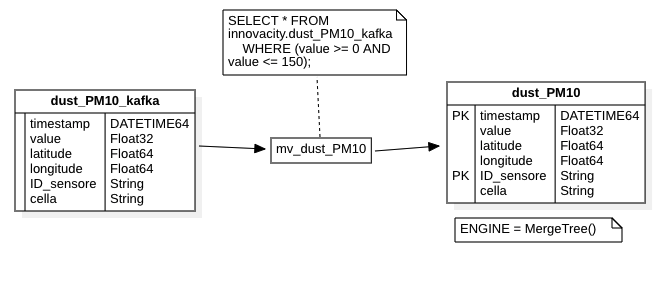
\includegraphics[width=1\textwidth]{../Images/SpecificaTecnica/dust_PM10.png}
    \caption{Tabella dust\_PM10\_kafka e dust\_PM10}
    \label{fig:dust_table}
\end{figure}

\paragraph{Projections per misurazioni di polveri sottili} 
Dopo aver considerato le stesse argomentazioni presentate nella sezione \ref{sec:temp_projections} riguardanti le misurazioni di temperatura, abbiamo deciso di estendere l'utilizzo delle projection anche alle misurazioni di polveri sottili. I vantaggi ottenuti risultano essere simili a quelli evidenziati per le misurazioni di temperatura, come descritto nella stessa sezione. A seguire, vengono illustrate le configurazioni delle projection relative alle tabelle delle misurazioni di polveri sottili:

\begin{lstlisting}
  --Projection per tabella dust_PM10
  ALTER TABLE innovacity.dust_PM10 ADD PROJECTION dust_sensor_cell_projection (SELECT * ORDER BY cella);
  ALTER TABLE innovacity.dust_PM10 MATERIALIZE PROJECTION dust_sensor_cell_projection;
\end{lstlisting}

\paragraph{Partition \& TTL per misurazioni di polveri sottili}
La configurazione riguardante il partizionamento e il TTL per le misurazioni di dust\_PM10 corrisponde a quella descritta nella sezione \ref{sec:temp_TTL} e \ref{sec:temp_part} in merito alle misurazioni di temperatura.
%_____________________________________________________________________________
\subsubsection{Misurazioni isole ecologiche}
Le considerazioni concernenti l'archiviazione delle misurazioni delle isole ecologiche corrispondono a quelle espresse nella sezione \ref{sec:misurazioni_temperatures} in merito alle misurazioni di temperatura. Il tipo della colonna \textit{value} è \textit{Float32} poichè il valore della misurazione riguarda la percentuale di riempimento, compreso tra 0 e 100. Le altre colonne sono identiche a quelle della tabella 'temperatures' e sono definite con lo stesso tipo di dato per garantire la precisione e l'integrità dei dati.

\begin{figure}[H]
	\centering
	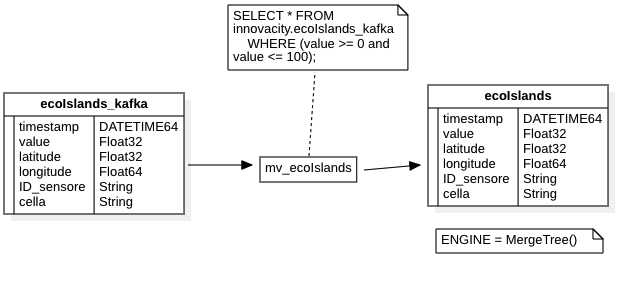
\includegraphics[width=1\textwidth]{../Images/SpecificaTecnica/ecoIslands.png}
	\caption{Tabella ecoIslands\_kafka e ecoIslands}
	\label{fig:ecoIslands_tables}
\end{figure}

\paragraph{Projections per misurazioni delle isole ecologiche} 
Dopo aver considerato le stesse argomentazioni presentate nella sezione \ref{sec:temp_projections} riguardanti le misurazioni di temperatura, abbiamo deciso di estendere l'utilizzo delle projection anche alle misurazioni delle isole ecologiche. I vantaggi ottenuti risultano essere simili a quelli evidenziati per le misurazioni di temperatura, come descritto nella stessa sezione. A seguire, vengono illustrate le configurazioni delle projection relative alle tabelle delle misurazioni delle isole ecologiche:

\begin{lstlisting}
  --Projection per tabella ecoIslands
	ALTER TABLE innovacity.ecoIslands ADD PROJECTION umd_sensor_cell_projection (SELECT * ORDER BY cella);
	ALTER TABLE innovacity.ecoIslands MATERIALIZE PROJECTION umd_sensor_cell_projection;
\end{lstlisting}

\paragraph{Partition \& TTL per misurazioni di umidità}
La configurazione riguardante il partizionamento e il TTL per le misurazioni di riempimento delle isole ecologiche corrisponde a quella descritta nella sezione \ref{sec:temp_TTL} e \ref{sec:temp_part} in merito alle misurazioni di temperatura.


\subsubsection{Misurazioni guasti elettrici} \label{sec:tab_guasti}
Le considerazioni concernenti l'archiviazione delle misurazioni dei guasti elettrici corrispondono a quelle espresse nella sezione \ref{sec:misurazioni_temperatures} in merito alle misurazioni di temperatura.
Il tipo della colonna \textit{value} è \textit{UInt8} poichè il valore delle misurazioni dei guasti elettrici è binario, 0 (guasto rilevato) oppure 1 (guasto non rilevato).

La tabella di destinazione \textit{ClickHouse}\textsubscript{\textit{G}} è nominata ‘electricalFault’:
Le altre colonne sono identiche a quelle della tabella 'temperatures' e sono definite con lo stesso tipo di dato per garantire la precisione e l'integrità dei dati.

\begin{figure}[H]
    \centering
    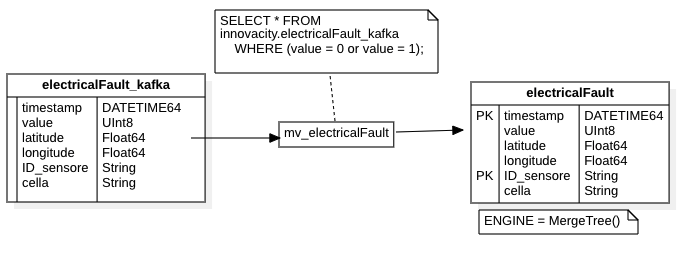
\includegraphics[width=1\textwidth]{../Images/SpecificaTecnica/electricalFault.png}
    \caption{Tabella electricalFault\_kafka e electricalFault}
    \label{fig:electricalFault_tables}
\end{figure}

\paragraph{Considerazioni su projection, partition e TTL per misurazioni di guasti elettrici} 
Le proiezioni per questo tipo di misurazione non offrono la stessa utilità rispetto a quelle relative a sensori con misurazioni non binarie, dove spesso si eseguono analisi temporali su ampi periodi e grandi volumi di dati filtrati per cella.

In questo contesto di misurazione, le operazioni di selezione sulla tabella si concentrano sul recupero dell'ultimo valore registrato.

La creazione di una proiezione per questa tabella comporterebbe solo un sovraccarico di calcolo e spazio su disco utilizzato, senza un reale vantaggio in termini di prestazioni o funzionalità.

Inoltre non si verificano le condizioni che giustifichino l'utilizzo del partizionamento e del TTL, in quanto non avrebbe senso aggregare misurazioni di questo genere dopo un certo periodo di tempo che porterebbero a misurazioni prive di valore informativo o senza significato.

\subsubsection{Misurazioni stazioni di ricarica}

Le considerazioni concernenti l'archiviazione delle misurazioni delle stazioni di ricarica corrispondono a quelle espresse nella sezione \ref{sec:tab_guasti} in merito alle misurazioni guasti elettrici.

Il tipo della colonna \textit{value} è \textit{UInt8} poichè il valore delle misurazioni delle stazioni di ricarica è binario, 0 (stazione di ricarica non occupata) oppure 1 (stazione di ricarica occupata).

La tabella di destinazione \textit{ClickHouse}\textsubscript{\textit{G}} è nominata ‘chargingStation’:

\begin{figure}[H]
    \centering
    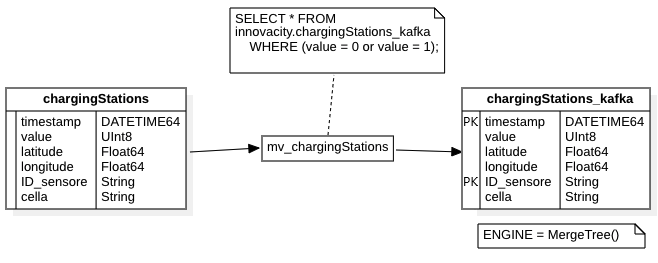
\includegraphics[width=1\textwidth]{../Images/SpecificaTecnica/chargingStations.png}
    \caption{Tabella chargingStation\_kafka e chargingStation}
    \label{fig:chargingStation_tables}
\end{figure}

\subsubsection{Misurazioni sensori di rilevameno dell’acqua}
Le considerazioni concernenti l'archiviazione delle misurazioni dei sensori di livello dell'acqua corrispondono a quelle espresse nella sezione \ref{sec:tab_guasti} in merito alle misurazioni guasti elettrici. Il tipo della colonna \textit{value} è \textit{UInt8} poichè il valore delle misurazioni dei sensori di livello dell'acqua è binario, 0 (acqua non rilevata) oppure 1 (acqua rilevata).

La tabella di destinazione \textit{ClickHouse}\textsubscript{\textit{G}} è nominata ‘waterPresence’:

\begin{figure}[H]
	\centering
	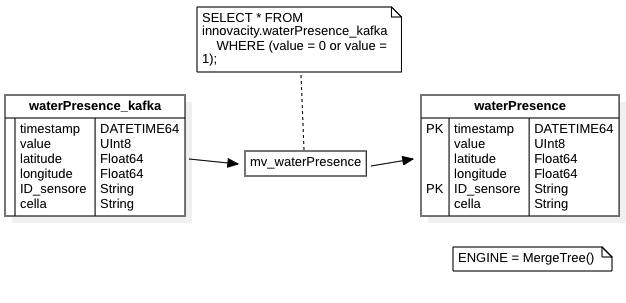
\includegraphics[width=1\textwidth]{../Images/SpecificaTecnica/waterPresence.png}
	\caption{Tabella waterPresence\_kafka e waterPresence}
	\label{fig:waterPresence_tables}
\end{figure}


\subsubsection{Punteggi di salute}
Viene creata anche una tabella dedicata alla persistenza dei punteggi di salute nel tempo calcolati per ogni cella della città. La tabella di destinazione \textit{ClickHouse}\textsubscript{\textit{G}} è nominata ‘healthScore’, i campi sono: cella (String), value (Float32), timestamp(DATETIME64).


\begin{figure}[H]
  \centering
  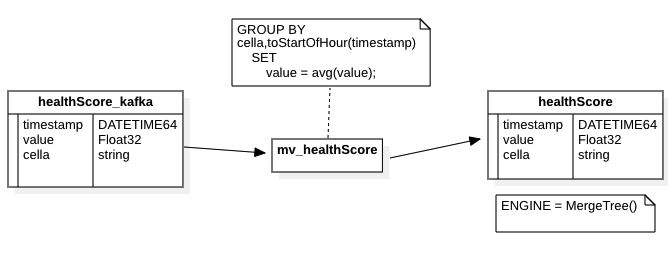
\includegraphics[width=1\textwidth]{../Images/SpecificaTecnica/healthScore.png}
  \caption{Tabella healthScore\_kafka e healthScore}
  \label{fig:HealthScore_tables}
\end{figure}

\paragraph{Time to Live punteggio di salute}
La tabella dedicata alle misurazioni di salute include la configurazione di un TTL che consente l'aggregazione dei dati dopo un mese dal timestamp della misurazione in una singola misurazione per cella e per ora.

Questo approccio consente di ridurre l'utilizzo dello spazio di archiviazione e accelerare il tempo di interrogazione, mantenendo comunque un livello di dettaglio adeguato per le analisi.
 